\documentclass{beamer}
\usetheme{metropolis}
\usepackage{graphicx}
\usepackage{booktabs}
\usepackage{hyperref}
\usepackage{listings}
\colorlet{shadecolor}{gray!40}

\lstset{
	language=R,
	basicstyle=\ttfamily\small,
	commentstyle=\color{black},
	keywordstyle=\color{blue},
	numbers=left,
	numberstyle=\tiny\color{red},
	stepnumber=1,
	numbersep=5pt,
	backgroundcolor=\color{shadecolor},
	showspaces=false,
	showstringspaces=false,
	showtabs=false,
	frame=single,
	tabsize=2,
	captionpos=b,
	breaklines=true,
	breakatwhitespace=false,
	title=\lstname
}


\newenvironment{bigitemize}{\itemize\addtolength{\itemsep}{10pt}}{\enditemize}
\newcommand\independent{\protect\mathpalette{\protect\independenT}{\perp}}
\def\independenT#1#2{\mathrel{\rlap{$#1#2$}\mkern2mu{#1#2}}}
\title{Microeconometrics Module}
\subtitle{Lecture 4: Selection Bias}
\author{Swapnil Singh}
\date{Lietuvos Bankas and KTU \\ \href{https://github.com/swapnil1987/econometrics-2024}{\textcolor{magenta}{Course Link}}}

\begin{document}
	
	\maketitle
	
	
	
	\begin{frame}
		\frametitle{Health Insurance and Health}
		\begin{itemize}
			\item \textbf{Question:} Does provision of health insurance improves health outcomes?
			\item ``Other things equal'' question: contrasting the health of someone with insurance coverage to the same person 
			\item We arrive at the fundamental problem of causal inference
			\begin{itemize}
				\item either people are insured or they are not
				\item you cannot observe both simultaneously
			\end{itemize}
		\end{itemize}
	\end{frame}
	
	
	\begin{frame}
		\frametitle{National Health Interview Survey (NHIS)}
		\begin{itemize}
			\item Conducted by National Center for Health Statistics (NCHS)
			\item Primary source of information on individual's health living in US
			\item Questions are asked related to medical conditions, health insurance, doctor's office visits, physical activity etc.
		\end{itemize}
	\end{frame}
	
	\begin{frame}
		\frametitle{National Health Interview Survey (NHIS)}
		\begin{figure}
			\centering
			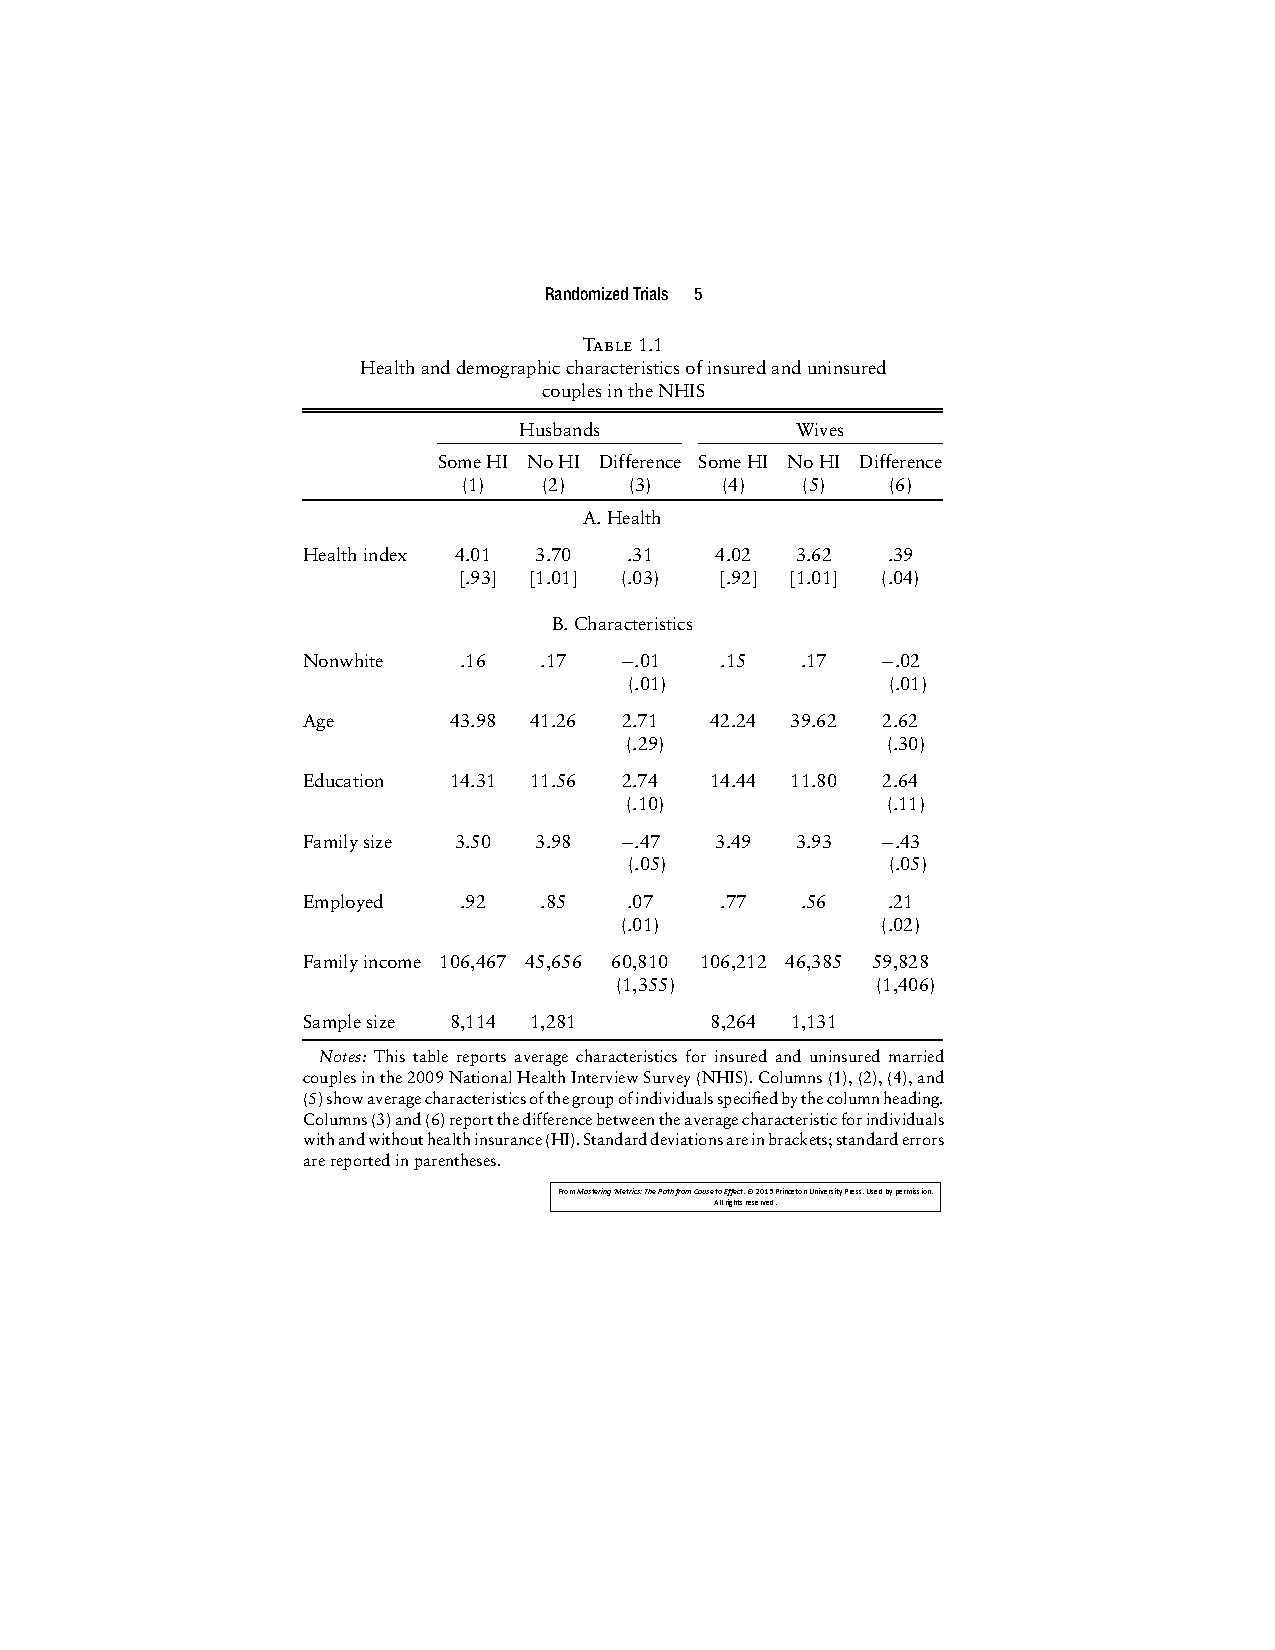
\includegraphics[ height=\textheight]{figures/MMtbl11}
		\end{figure}
	\end{frame}
	
	\begin{frame}
		\frametitle{Simpler Example}
		\begin{figure}
			\centering
			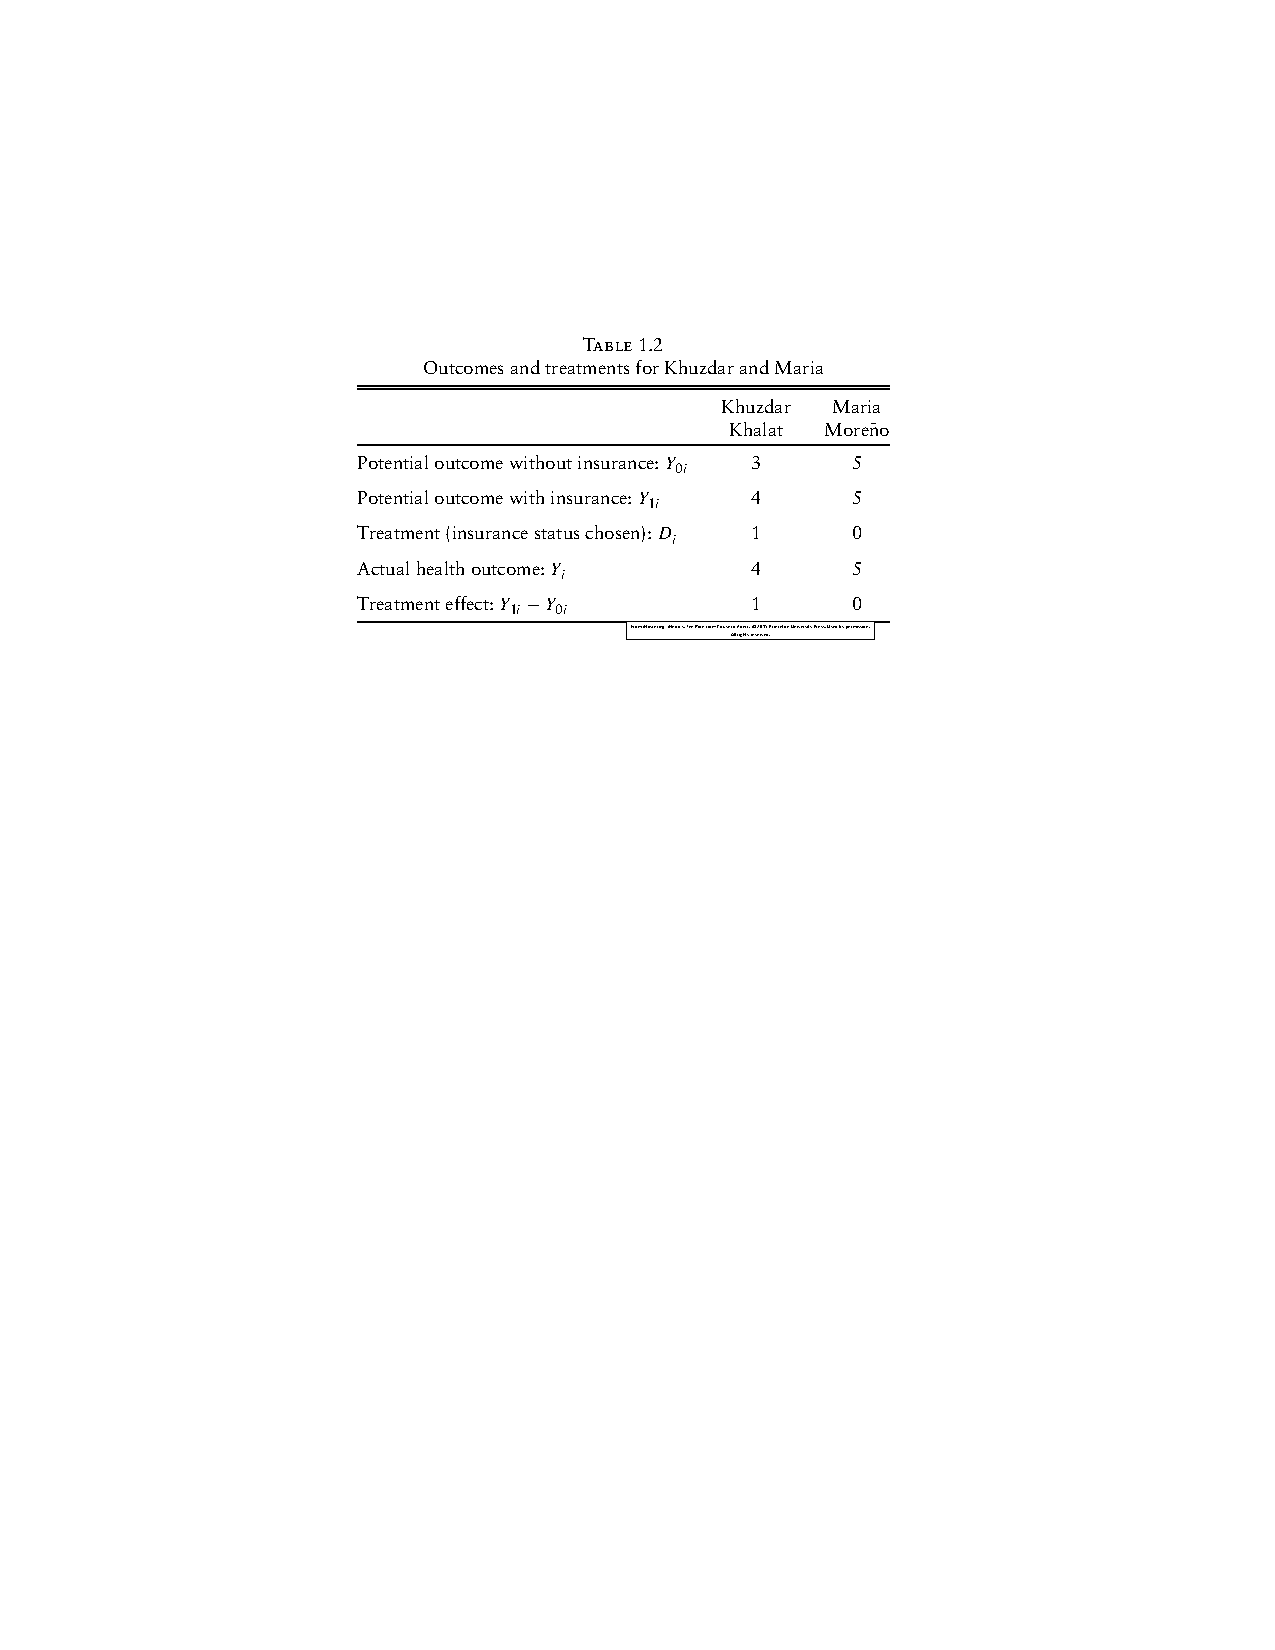
\includegraphics[ width=\textwidth]{figures/MMtbl12}
		\end{figure}
	\end{frame}
	
	\begin{frame}
		\frametitle{Simpler Example}
		\begin{itemize}
			\item Khuzdar takes the insurance
			\item Maria does not take the insurance
			\item Hence:
			\begin{align*}
				Y_{Khuzdar} &= Y_{Khuzdar,1} = 4\\
				Y_{Maria} &= Y_{Maria,0} = 5\\
			\end{align*}
			\item $Y_{Khuzdar} - Y_{Maria} = 4-5 = -1$
			\item Health insurance negatively affects health standard
			\item Wait a minute! What?
		\end{itemize}
	\end{frame}
	
	\begin{frame}
		\frametitle{Simpler Example}
		\small
				\begin{itemize}
			\item Comparison between Khuzdar and Maria's health is not a good comparison. Why?
			\begin{align*}
				Y_{Khuzdar} - Y_{Maria} &= Y_{Khuzdar,1} - Y_{Maria, 0}\\		
				&= \underbrace{Y_{Khuzdar,1} - Y_{Khuzdar,0}}_{\text{causal effect}} + \underbrace{Y_{Khuzdar,0} - Y_{Maria, 0}}_{\text{selection bias}}\\
				&= 4 - 3 + 3 - 5\\
				&= 1 - 2\\
				&= -1    
			\end{align*}
			\item So causal effect of health insurance is positive
			\item But selection bias, which captures the difference in health if both of them had decided to go without insurance, dominates
			\item In other words: the health of Khuzdar was worse than Maria to begin with. Hence comparing the (treated) health of Khuzdar with (untreated) health of Maria is not a fair comparison
		\end{itemize}
	\end{frame}
	
	\begin{frame}
		\frametitle{Further Notations and Generalizations}
		\small
		\begin{itemize}
			\item Suppose there are $n$ individuals
			\item Some get health insurance and some don't
			\item Construct a dummy variable $D$ such that
			\begin{align*}
				D_i = \left\{\begin{array}{cc}
					1 & \text{if} \;\; i \;\; \text{is insured}\\
					0 & \text{otherwise}\\
				\end{array} \right.
			\end{align*}
			\item Further assume that access to health insurance affects health standard by $\kappa$ 
			$$ Y_{1i} = Y_{0i} + \kappa$$
			\item Then difference in health status of insured versus uninsured is
			\begin{align*}
				&\Rightarrow Avg_n[Y_i| D_i = 1] - Avg_n[Y_i| D_i = 0]\\
				&\Rightarrow Avg_n[Y_{1i}| D_i = 1] - Avg_n[Y_{0i}| D_i = 0]\\
				&\Rightarrow Avg_n[\kappa + Y_{0i}| D_i = 1] - Avg_n[Y_{0i}| D_i = 0]\\
				&\Rightarrow \underbrace{\kappa}_{\text{causal effect}} + \underbrace{Avg_n[Y_{0i}| D_i = 1] - Avg_n[Y_{0i}| D_i = 0]}_{\text{selection bias}}\\
			\end{align*}
		\end{itemize}
	\end{frame}
	
	\begin{frame}
		\frametitle{Summary}
		\begin{itemize}
			\item Differences in group means = average causal effect + selection bias
			\item How can we be sure that there is selection bias?
			\item Let's have a look at Table 1.1 again
		\end{itemize}
	\end{frame}
	
	\begin{frame}
		\frametitle{National Health Interview Survey (NHIS)}
		\begin{figure}
			\centering
			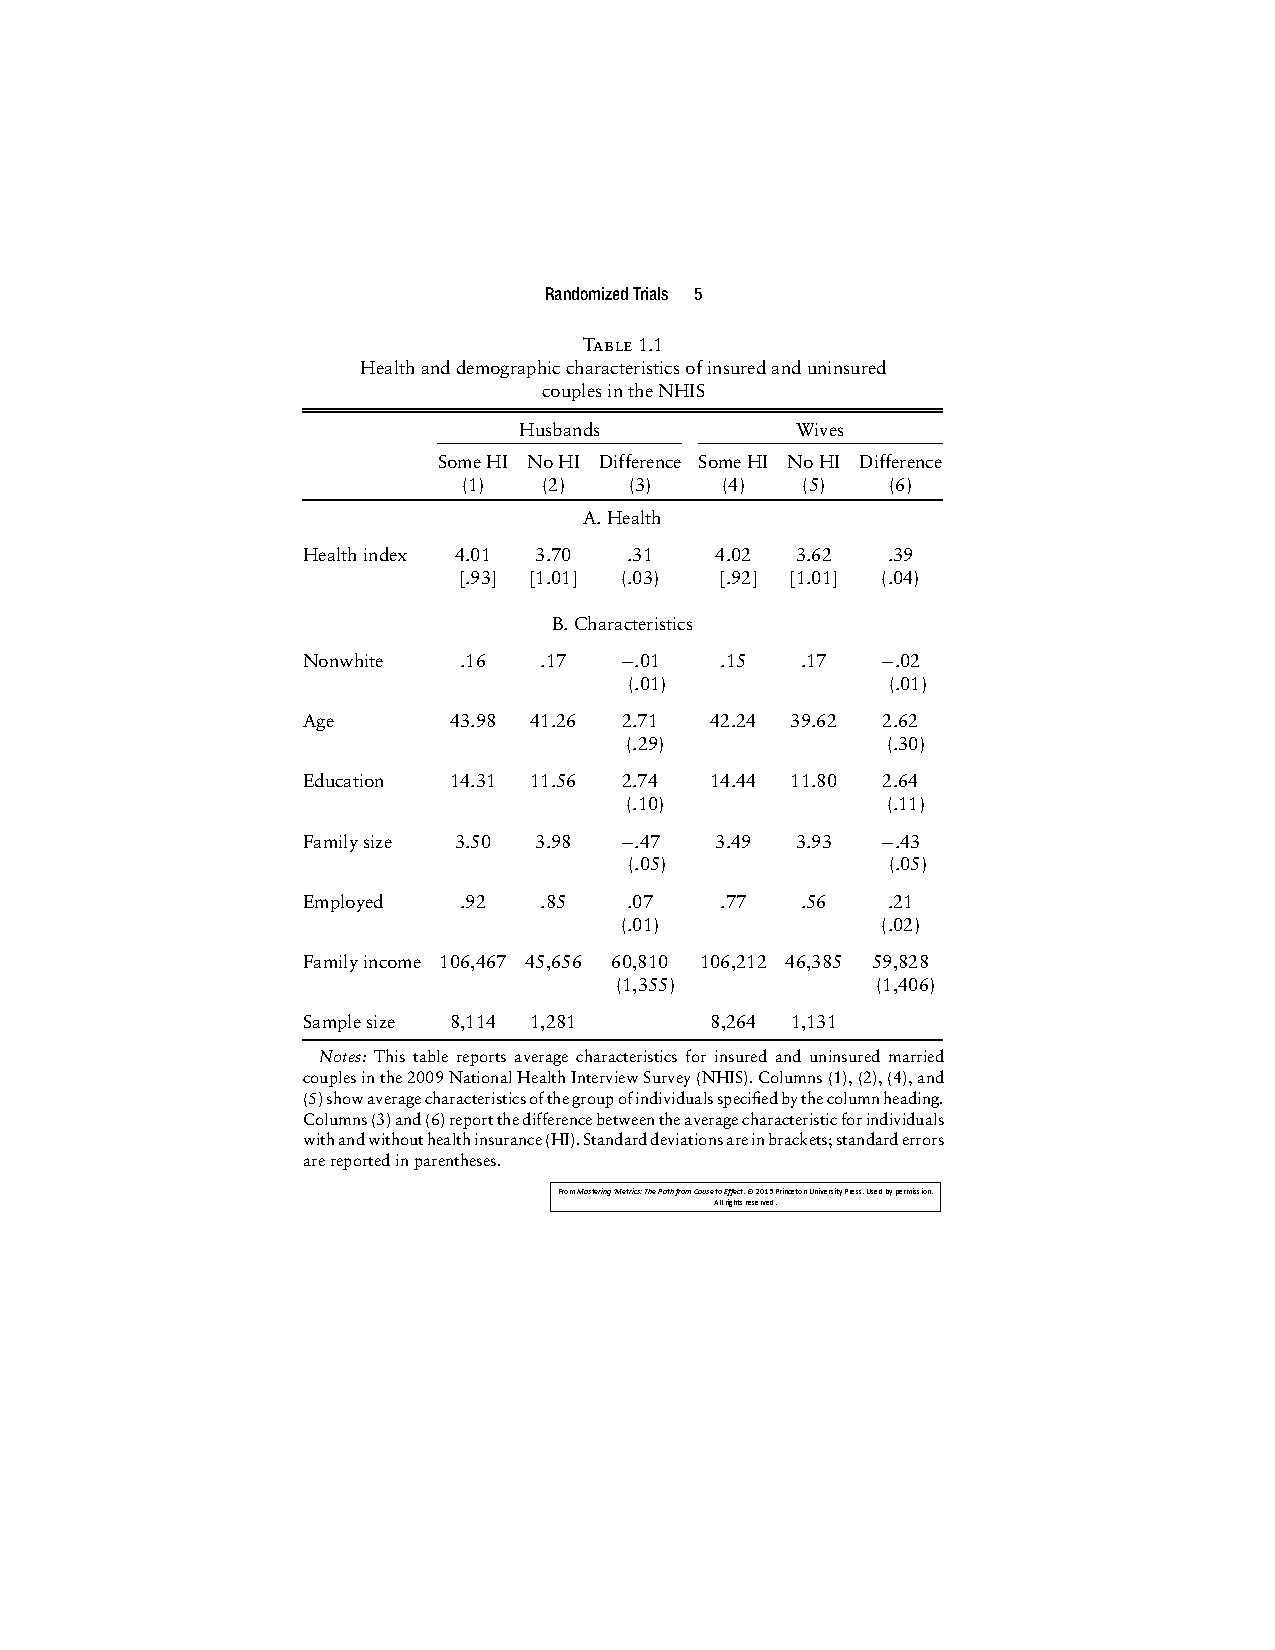
\includegraphics[ height=\textheight]{figures/MMtbl11}
		\end{figure}
	\end{frame}
	
	\begin{frame}
		\frametitle{Summary}
		\begin{itemize}
			\item Differences in group means = average causal effect + selection bias
			\item How can we be sure that there is selection bias?
			\item Let's have a look at Table 1.1 again
			\begin{itemize}
				\item insured people are also more educated
				\item hence, maybe, education is also playing a role
			\end{itemize}
			\item So, in short, selection bias does not allow us to compare apples to apples
			\item ``Other things'' are really not equal
		\end{itemize}
	\end{frame}
	
	\begin{frame}
		\frametitle{Observed versus Unobserved Differences}
		\begin{itemize}
			\item Table 1.1 shows that insured and uninsured people differ in observable ways
			\item But people can (and do) differ in unobservable ways
			\begin{itemize}
				\item $A$ and $B$ are twins
				\item Both have same education, age and occupation
				\item However, $A$ loves sweets but $B$ doesn't
				\item Sugar eating habits are not observed
			\end{itemize}
			\item Point is that there can still be selection bias even if observables are not different
		\end{itemize}
	\end{frame}




	
\end{document}